\chapter{Experiment and Results} \label{chapter4}

\section{Experiments on System Call Data set}
\label{sec:experiments}

We evaluate the accuracy and efficiency of our pruning techniques using a modern system call dataset, called ADFA Linux Data set (ADFA-LD), which has been recently made publicly available on the website of the University of New South Wales \cite{Creech2013a}.
The ADFA-LD data set is generated by exploiting various security vulnerabilities in a Ubuntu operating system (OS) hosting a web server.
The systems consists of a fully patched Ubuntu Linux 11.04 OS with an Apache 2.2.17 web server, PHP 5.3.5 server side scripting engine, TikiWiki 8.1 content management system, FTP server, MySQL 14.14 database management system and an SSH server.
First they collect normal system call traces by letting users perform basic operations, such as web browsing and Latex document preparations under controlled situations.
The anomalous system call traces are collected while the system is being under six types of attack vectors resulting in a total of 60 attacks.
These attacks were launched by a certified penetration tester against the system and included web-based exploitation, simulated social engineering, poisoned executable, remotely triggered vulnerabilities, remote password brute-force attacks and system manipulation.
The authors of the ADFA-LD have organized the data set into 833 normal traces for training the anomaly detectors, and 4373 normal traces and 60 anomalous traces for testing.

In our experiments, we used the following experimental setup.
First, we trained 20 HMMs with different numbers of states (i.e., $K=20$ soft detectors), using the 833 normal traces provided for training in the ADFA-LD data set.
On average, the output of each HMM is thresholded into $n_{avg} = 100$ thresholds or crisp detectors, which provides $n = K \times n_{avg} = 20\times 100 =2000$ crisp detectors in the ensemble.

The objective is to choose the most accurate subset from this ensemble for combination while pruning the remaining detectors according to our MinMax-Kappa or ROCCH-Kappa technique.
Then, the ROC curves and AUC results are compared to those of IBC and the pairwise Bruteforce Boolean Crisp combination (BBC2).
BBC2 is another baseline, which is the PBC Algorithm~\ref{PBC}, but without any pruning mechanism.

For evaluation of performance, a 5-fold cross-validation (5FCV) is applied to the test set comprising the 4373 normal and the 60 anomalous traces.
Since the number of anomalous traces is relatively small with reference to the normal ones, we applied the cross validation to partition the normal and anomalous sets separately, such that we keep the same ratio (normal to anomalous) and guarantee that all folds include the anomalies.
Accordingly, each fold contains 874 traces selected at random from the 4373 normal traces and 12 attacks traces selected at random from the 60 attack traces.

In contrast with the standard way of applying the 5FCV, we used one fold for computing the Boolean combination according to each of the combination technique,
and the remaining four folds (i.e., 3498 normal traces and 48 attack traces) are used for evaluating and benchmarking the detection performance.
This is because we wanted to test the boost in performance while using a small number of anomalies during combination. The reuslt are shown in section~\ref{sec:results-ADFA}.

For the second data set, we used the Canali data set~\cite{Canali2012}. The data was generated from 10 different machines. Our models, which are 4 HMMs and 5 SVMs, are trained on the normal data from: anubis-good + machine1 + ... + machine9, and the scores that we used are computed on the test data: machine10 that consist of (23 normal traces) + malware (5855 anomalous traces).

With this data set, in contrast with ADFA that we showed the boost in result with a small number of anomalies we want to show even when  anomalies are the majority of the test set with PBC technique there is a boost in result.
Here again we applied the PBC technqie with help of different distance correlation metric (Kappa, Distance Covariance, Distance Correlation) and compare the result with BBC2 and IBC. For Canali we used 5FCV approach as well. The reuslt are shown in section~\ref{sec:results-canali}.



\section{Results (ADFA)}
\label{sec:results-ADFA}



\begin{figure}[t]
\centering
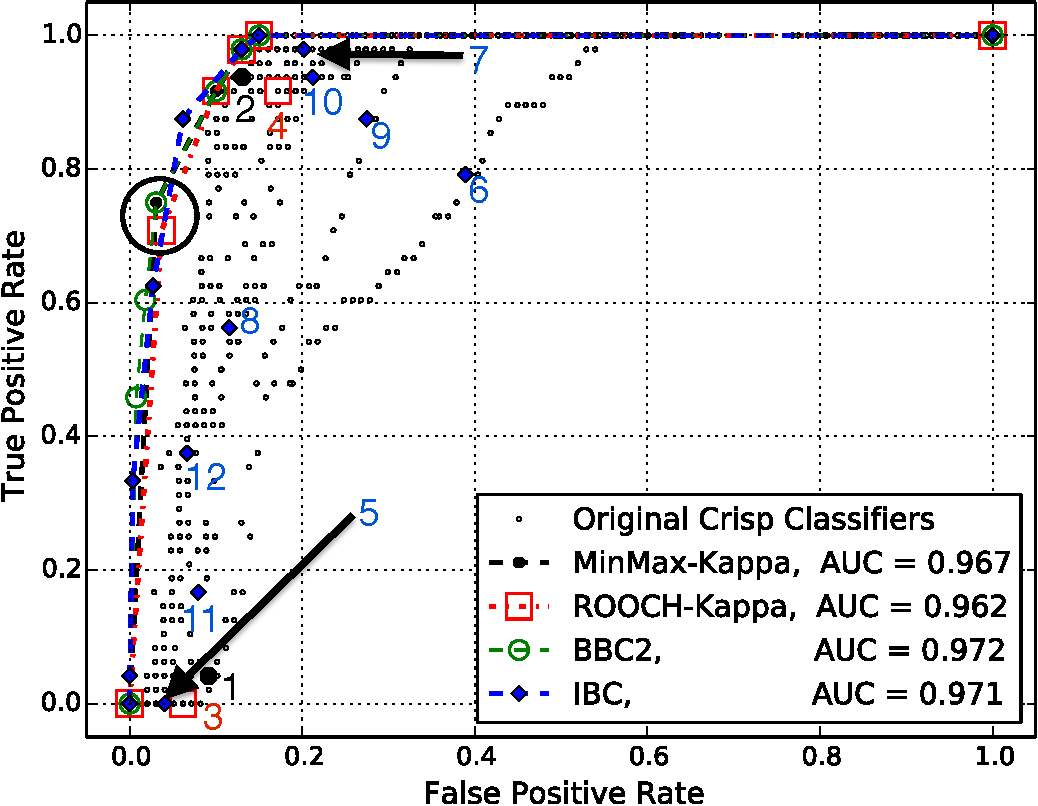
\includegraphics[width=\columnwidth]{figs/roc_curves_testing_fold3}
\caption{One of the ROC curves results of 5-folds cross-validation of Boolean combination on one fold and evaluated on four folds. The numbers represent the crisp detectors selected for combination (by each technique) to achieve about the same operational point as denoted by the large black circle}
\label{fig:roc_curves}
\end{figure}

\begin{figure}[t]
\centering
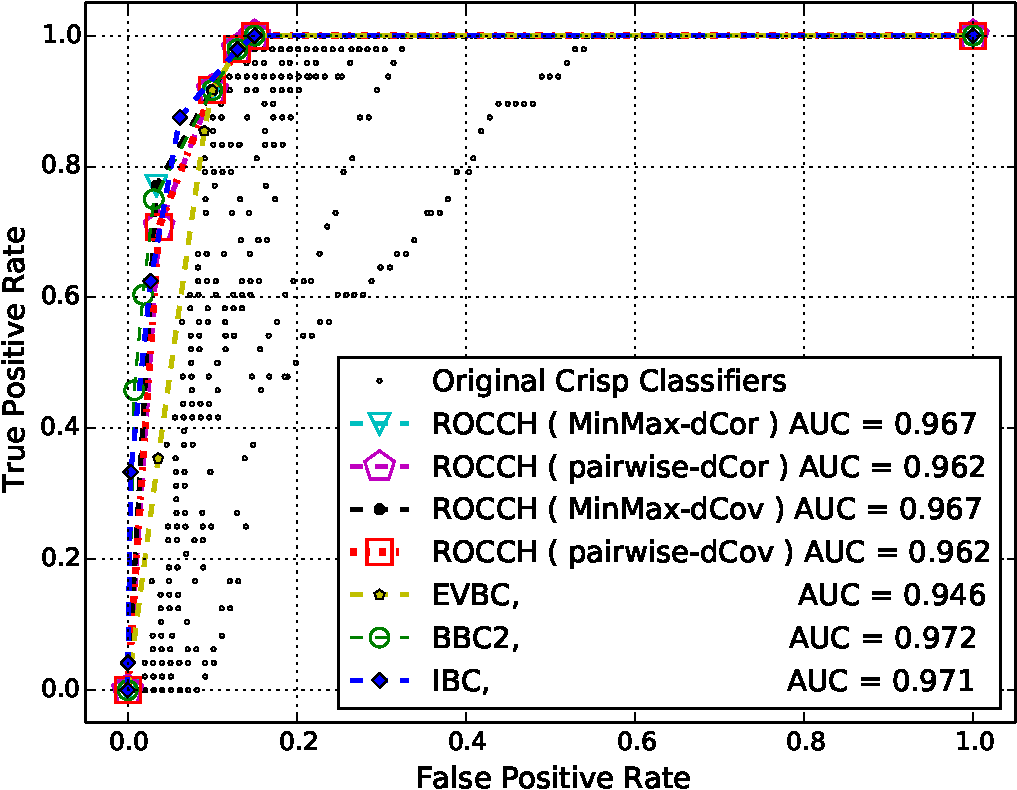
\includegraphics[scale=0.85]{figs/ADFA-dcov/IBC_BCC_Pruned_Classifier_ConvexHull_withoutRandom_validation}
\caption{The same ROC curves results of 5-folds cross-validation of Boolean combination on one fold and evaluated on four folds that was used in Figure~\ref{fig:roc_curves} with other distance correlation metrics}
\label{fig:roc_curves_dcov}
\end{figure}



\begin{table}[b]
    \centering
    \renewcommand{\arraystretch}{1.3}
    \caption{Average AUC values and their standard deviations over the 5FCV for each techniques. Design on one fold and evaluated on four folds. }
    \label{tab:auc}
    \centering
    \scalebox{1.2}{
    \begin{tabular}{lrr}
        \hline
        Method Name & Mean & Std\\
        \hline
        \hline
        BBC2 & 0.97426 & 0.001  \\
        IBC & 0.97276 & 0.001  \\
        MinMax-Kappa & 0.97074 & 0.003  \\
        ROCCH-Kappa & 0.97051 & 0.003  \\
        EVBC & 0.94472 & 0  \\
        MinMax-dCor & 0.9673 & 0.006  \\
        ROCCH-dCor &  0.97067 & 0.005 \\
        MinMax-dCov & 0.96515 & 0.004  \\
        ROCCH-dCov &  0.97051 & 0.005  \\
        \hline
    \end{tabular}}
\end{table}

\begin{table}[b]
    % \normalsize
    \small
    \centering
    \renewcommand{\arraystretch}{1.3}
    \caption{Comparison of pruning and combination time (seconds) and number of Boolean operations required to achieve the final ROCCH during the design phase, and the number of selected detectors during the operational phase. All values are averaged over 5FCV.}
    \label{tab:time-complexity}
    \centering
    \scalebox{1}{
    \begin{tabular}{lrrr|r}
    % \begin{tabular}{L{1.8cm}rrr|r}
        & \multicolumn{3}{c}{\bf Design Phase } & \bf Operations \\
        \cline{2-5}
        Method &   Pruning &  Combination &  \# Boolean &  \# Combined\\
        Name &     Time    &  Time &  operations & detectors\\
        \hline
        \hline
        BBC2            & N/A     & 16364 &   $4,000,000$ & 2\\ %1617
        IBC             & N/A     & 11    &   $11,000$  & 11 \\
        MinMax-Kappa    & 1.6   & 15    &   $19,701$    & 2\\
        ROCCH-Kappa     & 11.8  & 38    &  $37,701$     & 2 \\
        EVBC     & 370  &   13  &  $...$     & 2 \\
        MinMax-dCor    &   74 &   16  &   $19,701$    & 2\\
        ROCCH-dCor     & 190  &   30  &  $37,701$     & 2 \\
        MinMax-dCov    &   64 &    17 &   $19,701$    & 2\\
        ROCCH-dCov     & 185  &    37 &  $37,701$     & 2 \\
        \hline
    \end{tabular} }
\end{table}


Figure~\ref{fig:roc_curves} shows the ROC curves and the AUC performance for both pruning techniques proposed in this paper (MinMax- and ROCCH-Kappa) compared to those of IBC and BBC2 (PBC with no pruning mechanism). And Figure~\ref{fig:roc_curves_dcov} shows the same ROC (the same fold) for both MinMax- and ROCCH- technique with different distance correlation as discussed in section~\ref{sub:minmax-rocch-dcov}.

These results are for one of the 5FCV experiments (the combinations are computed on one fold and evaluated on four) as described in Section~\ref{sec:experiments}.
As shown in the figure the results are comparable both in term of AUC values and the shape of the ROC curves.
This is also confirmed in Table~\ref{tab:auc}, where the AUC values of each combination technique is averaged over the 5FCV experiments.

Table~\ref{tab:time-complexity} shows the average over the 5FCV of the  pruning time (for MinMax-Kappa,  ROCCH-Kappa, MinMax-dCor, MinMax-dCov, ROCCH-dCor, ROCCH-dCov), combination time, and number of Boolean operations required by each technique to achieve the final ROCCH (as shown in  Figure~\ref{fig:roc_curves} and  Figure~\ref{fig:roc_curves_dcov} for one fold).  

We set the maximum number of selected detectors to $U=50$ for all the above-mentioned techniques (this can be further optimized, but gave good trade-off between performance and time complexity).
Therefore, the input to these pruning techniques is $n=2000$ crisp detectors, while the output is a subset of a maximum size of $50$ detectors provided for Boolean combination (in PBC Algorithm).
MinMax-Kappa took about $1.6$ seconds in average to select the best subset, while ROCCH-Kappa took about ten times more due the $n_{ev}$ factor, which is described in Section~\ref{sub:complexity}, to prune the ensemble of $n=2000$ detectors.
Furthermore, MinMax-Kappa is able to select a smaller number of detectors than $U=50$ on average and computes the Kappa values once, which explains the reduction in combination time and number of Boolean operations compared to those of ROCCH-Kappa, as shown in Table~\ref{tab:time-complexity}.
Thereby, although both techniques provide similar AUC performance, MinMax-Kappa is slightly preferred due to its improved efficiency  compared to ROCCH-Kappa.

Table~\ref{tab:time-complexity} also shows that our MinMax-Kappa techniques was able to achieve the same AUC performance of BBC2 (the pairwise Boolean combination of the $2000$ detectors), by selecting less than $50$ detectors out of the $2000$ ones.
More interestingly, MinMax-Kappa achieved these results with an average time of three magnitudes lower than that of BBC2, and about 200 times fewer Boolean operations.

Compared to IBC, MinMax-Kappa requires, on average, slightly more combination time and a larger number of Boolean operations to achieve the same AUC performance.
However, the number of selected detectors and Boolean functions required to realize each vertex on the ROCCH is on average five times more according to our experiments.
For instance, to achieve the final operating points denoted with a  large black circle on Figure~\ref{fig:roc_curves}, MinMax-Kappa uses two detectors and one Boolean function according to the following formula:
\begin{equation*}
    \neg D_1 \oplus  D_2
\end{equation*}
Note that in Figure~\ref{fig:roc_curves}, we only shown the number of crisp detectors not to clutter the figures (i.e., 1 means $D_1$)
\\
Similarly, ROCCH-Kappa uses the following detectors and Boolean function to achieve similar operating point:
\begin{equation*}
    \neg D_3 \oplus  D_4
\end{equation*}
However to achieve similar point of operations, IBC requires eight detectors combined according to the following Boolean operations:
\begin{equation*}
    (((((((D_5 \oplus D_6) \land \neg D_{11})  \land D_7) \oplus D_8) \equiv D_9) \lor D_{10})  \land D_{12})
\end{equation*}

The average number of combined detectors on the final ROCCH over the 5FCV is about 10 detectors when using IBC compared to two detectors when using PBC with MinMax-Kappa pruning as shown in the last column of Table~\ref{tab:time-complexity}.
This sequence of combination rules grows linearly with the number of soft detector $K$, which makes IBC results difficult to analyse and understand for large $K$ values.
In contrast to IBC, the combination of two detectors according to combination of PBC with MinMax-Kappa are insensitive to order in which detectors are input to the algorithm, which makes the search for the best subset of detectors easier.
However, MinMax-Kappa requires an optimization of the maximum number of detectors $U$ that trades off the complexity and the accuracy.
Setting an ADS based on two HMMs into operations, requires less time and memory resources to provide the output probabilities of the input system call sequences.
In addition, operating a small number of detectors becomes critical in application of anomaly detection mobile security, due to the constraint on power resources.

%%%%%%%%%%%%%%%%%%%%%%%%%% 4 Folds results

\begin{figure}[t]
\centering
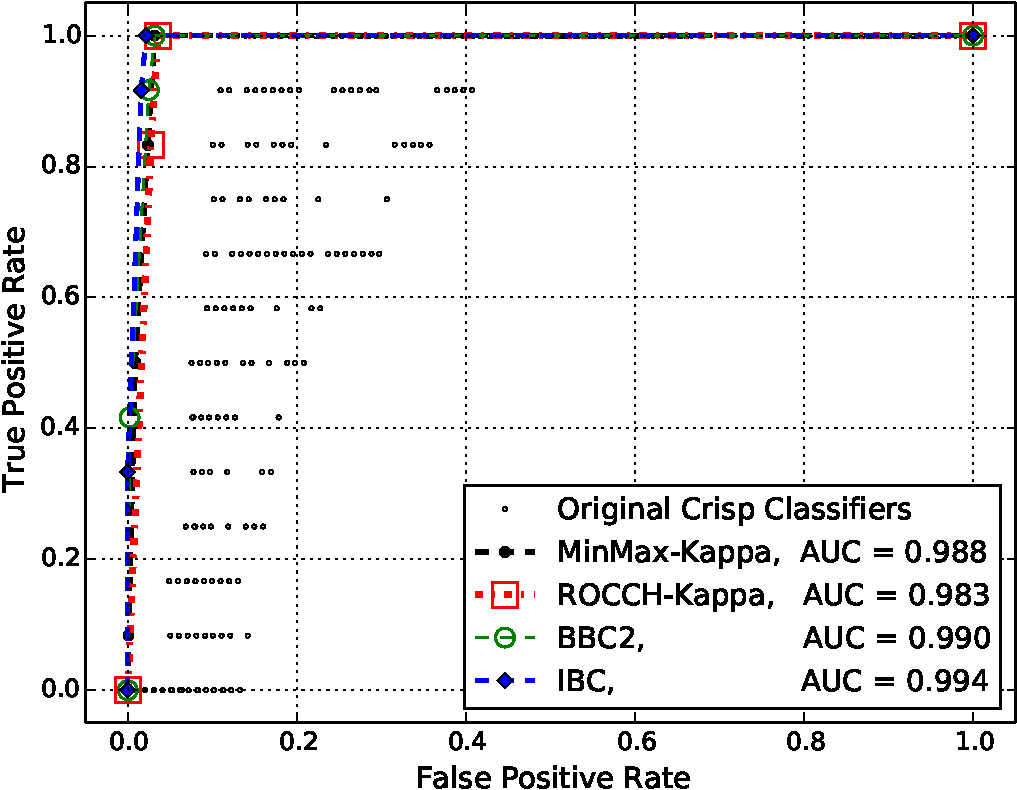
\includegraphics[width=\columnwidth]{figs/roc_curves_training_on_4_folds_testing_on_1-crop}
\caption{One of the ROC curves results of 5-folds cross-validation of Boolean combination on four folds and evaluated on one fold.}
\label{fig:roc_curves4}
\end{figure}

\begin{figure}[t]
\centering
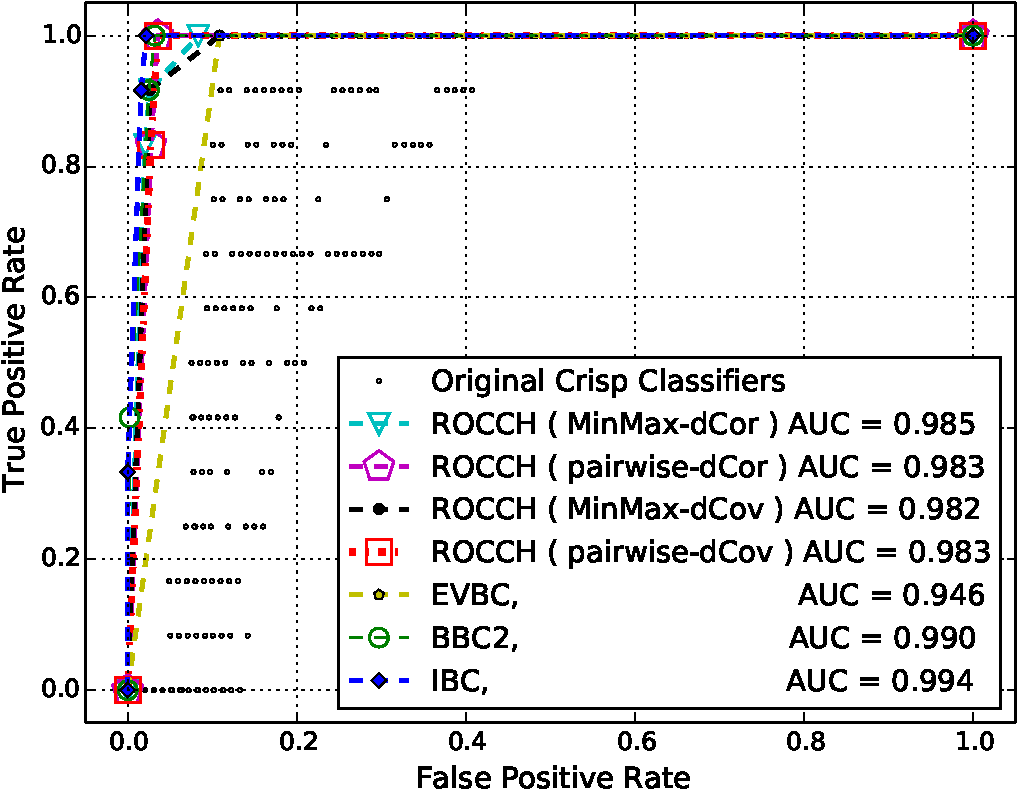
\includegraphics[width=\columnwidth]{figs/ADFA-dcov/IBC_BCC_Pruned_Classifier_ConvexHull_withoutRandom_validation_4fold}
\caption{The same ROC curves results of 5-folds cross-validation of Boolean combination on four folds and evaluated on one fold that was used in fig.~\ref{fig:roc_curves4} with other distance correlation metrics.}
\label{fig:roc_curves4_dcov}
\end{figure}




\begin{table}[b]
    \centering
    \renewcommand{\arraystretch}{1.3}
    \caption{Average AUC values and their standard deviations over the 5FCV for each techniques. Design on four folds and evaluated on one fold.  }
    \label{tab:auc4}
    \centering
    \scalebox{1.2}{
    \begin{tabular}{lrr}
        \hline
        Method Name & Mean & Std\\
        \hline
        \hline
        BBC2 & 0.98177 & 0.00636  \\
        IBC & 0.98003 & 0.01127  \\
        MinMax-Kappa & 0.97806 & 0.00640  \\
        ROCCH-Kappa & 0.97578 & 0.00585  \\
        EVBC & 0.94472 & 0  \\
        MinMax-dCor & 0.9725 & 0.012  \\
        ROCCH-dCor &  0.9752 & 0.005 \\
        MinMax-dCov & 0.96268 & 0.011  \\
        ROCCH-dCov &  0.9753 & 0.005  \\
        \hline
    \end{tabular}}
\end{table}

We conducted an alternative case study to check the impact on ROC and AUC performance of all Boolean techniques, when the number of anomalies is increased during the design phase.
Therefore, instead of using one fold (comprising $12$ attack traces and $874$ normal traces) for selecting the crisp detectors and the corresponding Boolean functions, as described in Section~\ref{sec:experiments}, we used 4 folds ($48$ attack traces and $3498$ normal traces) and one fold for evaluation of performance.

Figure~\ref{fig:roc_curves4} and figure~\ref{fig:roc_curves4_dcov} show the ROC curves and the AUC performance for all techniques, PBC with MinMax-Kappa, ROCCH-Kappa, MinMax-dCor, MinMax-dCov, ROCCH-dCor, ROCCH-dCov, IBC and BBC2.
Again, the presented results are for one of the 5FCV experiments (but the combinations are computed on four folds and evaluated on one).
As shown in the figure, all techniques provide comparable results; however, with a large improvement in detection accuracy over those presented in Figure~\ref{fig:roc_curves}.
For instance, for detecting all attacks ($tpr = 100\%$) the false positive rate is now $fpr\approx  2\%$ compared to $fpr\approx 16\%$ in Figure~\ref{fig:roc_curves}.
This boost in performance can be also seen in Table~\ref{tab:auc4} in terms of average AUC values for each combination technique over the 5FCV experiments.
The results of this experiments show, as expected, that when the system is provided with more normal or attack traces, the overall performance of all Boolean combination techniques improves.
In such cases, there is no need to retrain the original detectors (HMMs in our case), which is a time consuming process, but the design phase of Boolean combination techniques must be repeated.
This provides an advantage for IBC and PBC, since they are efficient in selecting the detectors for final operations.
However, our PBC approach will always provide two detectors for each emerging point on the ROCCH, which is less costly to operate and easier to analyse in real-world setting.

\section{Results (Canali)}
\label{sec:results-canali}

\begin{figure}[t]
\centering
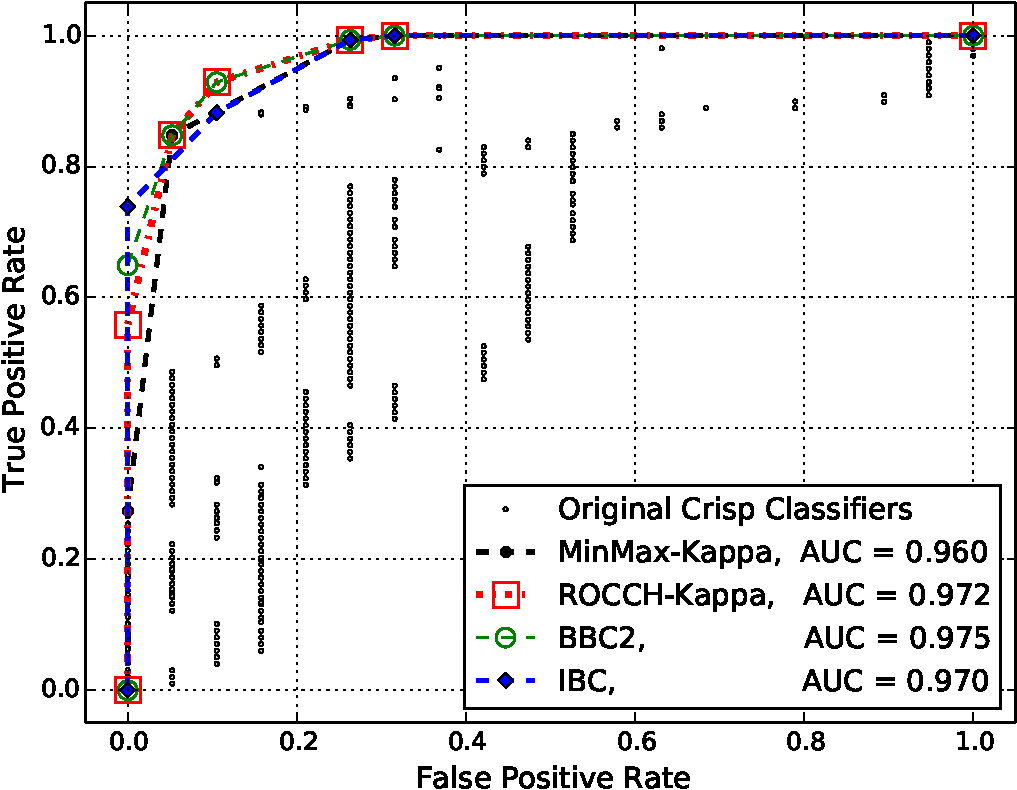
\includegraphics[width=\columnwidth]{figs/Canali/IBC_BCC_Pruned_Classifier_ConvexHull_withoutRandom_validation_4fold_kappa}
\caption{One of the ROC curves results of 5-folds cross-validation of Boolean combination on four folds and evaluated on one fold on Canali.}
\label{fig:roc_curves_canali}
\end{figure}

\begin{figure}[t]
\centering
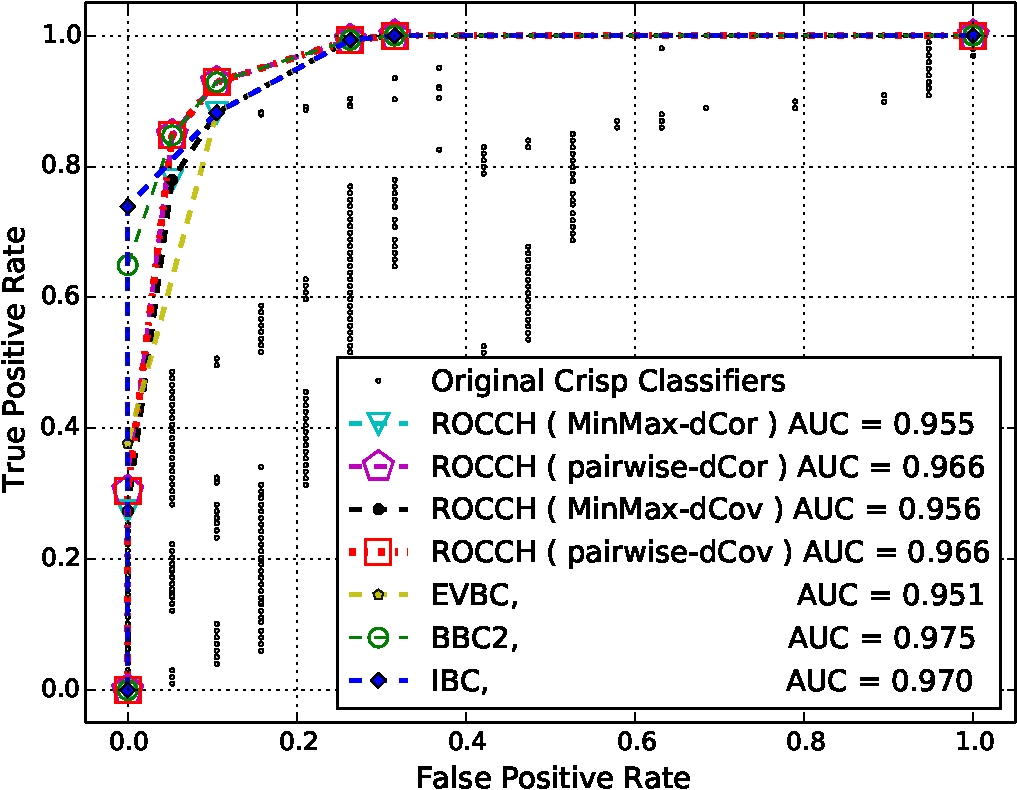
\includegraphics[width=\columnwidth]{figs/Canali/IBC_BCC_Pruned_Classifier_ConvexHull_withoutRandom_validation_4fold_dCov}
\caption{The same ROC curves results of 5-folds cross-validation of Boolean combination on one fold and evaluated on four folds that was used in Figure~\ref{fig:roc_curves_canali} with other distance correlation metrics}
\label{fig:roc_curves_dcov_canali}
\end{figure}



\begin{table}[b]
    \centering
    \renewcommand{\arraystretch}{1.3}
    \caption{Average AUC values and their standard deviations over the 5FCV for each techniques. Design on four folds and evaluated on one fold on Canali. }
    \label{tab:auc_canali}
    \centering
    \scalebox{1.2}{
    \begin{tabular}{lrr}
        \hline
        Method Name & Mean & Std\\
        \hline
        \hline
        BBC2 & 0.97398 & 0.008  \\
        IBC & 0.97141 & 0.006  \\
        MinMax-Kappa & 0.95884 & 0.005  \\
        ROCCH-Kappa & 0.9716 & 0.008  \\
        EVBC & 0.95074 & 0.006  \\
        MinMax-dCor & 0.95426 & 0.006  \\
        ROCCH-dCor &  0.96451 & 0.006 \\
        MinMax-dCov & 0.9616 & 0.011  \\
        ROCCH-dCov &  0.96451 & 0.006  \\
        \hline
    \end{tabular}}
\end{table}

Figure~\ref{fig:roc_curves_canali} shows the ROC curves and the AUC performance for both pruning techniques proposed in this paper (MinMax- and ROCCH-Kappa) compared to those of IBC and BBC2 (PBC with no pruning mechanism) on Canali data set in order to see if the PBC technique is consistent regardless of data set. And Figure~\ref{fig:roc_curves_dcov_canali} shows the same ROC (the same fold) for both MinMax- and ROCCH- technique with different distance correlation as discussed in section~\ref{sub:minmax-rocch-dcov}.

These results are for one of the 5FCV experiments (the combinations are computed on one fold and evaluated on four) as described in Section~\ref{sec:experiments}.
As shown in the figure the results are comparable both in term of AUC values and the shape of the ROC curves.
This is also confirmed in Table~\ref{tab:auc_canali}, where the AUC values of each combination technique is averaged over the 5FCV experiments.

In this experminet like what we did for ADFA~\ref{sec:results-ADFA} we set the maximum number of selected detectors to $U=50$ for all the above-mentioned techniques.
Therefore, the input to these pruning techniques is $n=900$ crisp detectors (4 different HMMS and 5 SVMs each thresholded 100 times), while the output is a subset of a maximum size of $50$ detectors provided for Boolean combination (in PBC Algorithm).

Compared to ADFA's~\ref{sec:results-ADFA} result here we can see that ROCCH-Kappa generate even better result than IBC, however the difference is not significant yet it persuade us more to use PBC; Since by using PBC we are guaranteed that our final formula is shorter and we have much fewer number of combinations that leads to less calculation time which saves CPU cycles (and get the result very much faster).

Running PBC as discussed~\ref{sec:pbc} with complettly new data set like Canali (which is for Widnows) and getting promising result is a proof that PBC technique is applicable on various data sets as long as having a diverse detectors trained on the them.

The key for PBC to work well is to have as many diverse detectors as possible. It doesn't matter if it's very complex detectors or simple one, we should have diverse pool of detctors; then with help of PBC we prune the pool to create the basket of detectors for combination. PBC with reasoble distance correlation tries to  select few sample from each set of detectors such that it represnts the original pool.

\section{Threats to Validity}
\label{sec:threat-validity}

A threat to internal validity exists in the implementation of the IBC, BBC2 and PBC algorithms as well as in conducting the experiments for anomaly detection.
We have mitigated this threat by manually verifying the outputs.

We have conducted experiments using only one system call data set derived from the Linux operating system, which consists a threat to external validity of this study.
More experiments are therefore required to generalize the presented results to other data sets, operating systems and other software vulnerabilities.

Evasion attacks could also pose a threat to validity.
For instance, \textit{mimicry} attacks try to mimic the normal system behavior will go undetected with the ADSs that are based on individual system calls or their temporal order \cite{Wagner2002}.
Mimicry attacks could be conducted by an attacker who is able to launch his attack without tempering the normal order of system calls by, for instance, replacing foreign system call sequences (which can be easily detected) with normal ones or by using system call arguments  \cite{Wagner2002}.

The manifestations of such mimicry attacks could be detected by including additional features, such as system call arguments \cite{Bhatkar2006}, return values extracted from the call stack information \cite{Feng2003}, and the user identity \cite{Larson2009}.
An added advantage of multiple detector systems, combined without our PBC, is that they can combine different detectors trained on various features, such as system call arguments, return values and other information flow features to help mitigating such evasion attacks.
